\chapter{Terminal building distribution}
	\section{Surface distribution}
	
	The terminal building interiors will be distributed according to the FAA criteria. This method has been chosen because it differentiates between domestic and international passenger flows, which are very well defined at this airport.
	
	\noindent In order to manage and distribute the space available, the forecasted traffic predicted in the prognosis is to be used.
	
	\noindent In first place, as shown in  table  \ref{FAAdomestic}, the surface corresponding to domestic traffic is distributed. According to prognosis data, the number of domestic passengers at design hour will be of 4850.
	
	\begin{table}[H]
	\centering
	\begin{tabular}{|c|c|c|c|}
	\hline
	\textbf{Surface} & \textbf{\% out of total} & \textbf{m2/pax} & \textbf{m2 total}\\
	\hline
	\textbf{Departures} & 0.0435 & 0.609 & 2953.65 \\
	\hline
	\textbf{Arrivals} & 0.0435 & 0.609 & 2953.65\\
	\hline
	\textbf{Waiting lobby} & 0.0739 & 1.035 & 5019.75\\
	\hline
	\textbf{Restrooms} & 0.013 & 0.183 & 887.55\\
	\hline
	\textbf{Kitchens} & 0.0652 & 0.913 & 4428.05 \\
	\hline
	\textbf{Restaurants} & 0.0652 & 0.913 & 4428.05\\
	\hline
	\textbf{Offices} & 0.1957 & 2.739 & 13284.15\\
	\hline
	\textbf{Other} & 0.0217 & 0.304 & 1474.4\\
	\hline
	\textbf{Circulation} & 0.4783 & 6.696 & 32475.6\\
	\hline
	\textbf{TOTAL} & & & \textbf{67904.85}\\
	\hline
	\end{tabular}
	\caption{Estimated surfaces according to FAA (domestic flights).}
	\label{FAAdomestic}
	\end{table}
	
	In second place, as shown in table \ref{table:FAAinternational}, the surface corresponding to international traffic is distributed. According to prognosis data, the number of international passenger at design hour will be of 3168.
	
	
	\begin{table}[H]
	\centering
	\begin{tabular}{|c|c|c|c|}
	\hline
	\textbf{Surface} & \textbf{\% out of total} & \textbf{m2/pax} & \textbf{m2 total}\\
	\hline
	\textbf{Departures} & 0.0435 & 0.609 & 2953.65 \\
	\hline
	\textbf{Arrivals} & 0.0435 & 0.609 & 2953.65\\
	\hline
	\textbf{Waiting lobby} & 0.0739 & 1.035 & 5019.75\\
	\hline
	\textbf{Restrooms} & 0.013 & 0.183 & 887.55\\
	\hline
	\textbf{Kitchens} & 0.0652 & 0.913 & 4428.05 \\
	\hline
	\textbf{Offices} & 0.1957 & 2.739 & 13284.15\\
	\hline
	\textbf{Other} & 0.0217 & 0.304 & 1474.4\\
	\hline
	\textbf{General circulation} & 0.307 & 6.145 & 19467.36\\
	\hline
	\textbf{Immigration} & 0.042 & 0.838 & 2654.78\\
	\hline
	\textbf{Customs} & 0.084 & 1.676 & 5309.57\\
	\hline
	\textbf{Health} & 0.028 & 0.559 & 1770.91\\
	\hline
	\textbf{Other checkpoints} & 0.006 & 0.112 & 354.816\\
	\hline
	\textbf{Circulation} & 0.198 & 3.966 & 12564.28\\
	\hline
	\textbf{TOTAL} & & & \textbf{63363.17}\\
	\hline
	\end{tabular}
	\caption{Estimated surfaces according to FAA (international  flights).}
	\label{table:FAAinternational}
	\end{table}
	
	Nevertheless, due to our airport structure and preliminary design, some of these areas are going to be shared between domestic and international passengers. This will allow to tighten the space and reduce the extension of the terminal building, which will be too extense for the number of passengers at design hour.
	
	Therefore, the final dimensioning of the airport will be as follows, shown in table \ref{table:FAAtotal}:
	
	\begin{table}[H]
	\centering
	\begin{tabular}{|c|c|c|c|c|c|}
	\hline
	\textbf{General (shared)} & \textbf{m2} & \textbf{Domestic} & \textbf{m2} & \textbf{International} & \textbf{m}2\\
	\hline
	\textbf{Departures} & 4725.56 & \textbf{Waiting lobby} & 5019.75 & \textbf{Immigration} & 2654.78\\
	\hline
	\textbf{Arrivals} & 4724.56 & \textbf{Circulation }& 32475.6 & \textbf{Customs} & 5309.57\\
	\hline
	\textbf{Restaurants} & 7082.83 & & & \textbf{Health} & 1770.91\\
	\hline
	\textbf{Offices} & 21248.50 & & & \textbf{Other checkpoints} & 354.81\\
	\hline
	\textbf{Other} & 2358.27 & & & \textbf{Circulation} & 12562.3\\
	\hline
	\textbf{Restrooms} & 1419.77 & & & \textbf{General circulation} & 19456.36\\
	\hline
	\textbf{Kitchens} & 7082.83 & & & \textbf{Waiting lobby} & 3009.60\\
	\hline
	\textbf{TOTAL} & \textbf{48641.34} & & \textbf{37495.35} & & \textbf{45131.33}\\
	\hline
	\end{tabular}
	\caption{Total surface distribution of terminal building.}
	\label{table:FAAtotal}
	\end{table}
	
	The total surface of the terminal building area, dedicated to passengers and airport management is of 131267 $\mathrm{m^2}$.
	
	\section{Dimensioning of elements}
\begin{enumerate}
\item \textbf{Check-in counters:} in order to define the check-in area, we have to determine the queueing area and the counters area. Considering the following parameters:
\begin{table}[H]
\centering
\begin{tabular}{|c|c|c|}
\hline
PHP(dep) & 2000 & 50\% for arrivals and departures\\
\hline 
b & 0 & Connecting pax not processed in airside\\
\hline
y & 20 min & Average ocuppation time\\
\hline 
s & 1.9 $\mathrm{m^2}$ & Recommended space by pax\\
\hline
o & 1.5 & Number of visitors for each pax\\
\hline 
t & 120 s & Average time of processed pax\\
\hline
\end{tabular}
\end{table}

\begin{figure}[H]
	\centering
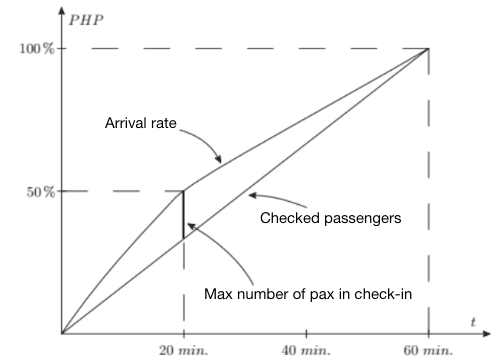
\includegraphics[width=10cm]{./images/graf1}
\caption{Plot PHP -- time.}
\end{figure}

Looking at the figure, it can be seen that the maximum number of checked-in passengers is 50\% in the first 20 min. Therefore:
\begin{align*}
\text{Fraction of total PHP} = \dfrac{PHP}{2}-\dfrac{PHP}{3}=\dfrac{PHP}{6}
\end{align*}

Therefore, the queueing area is of:
\begin{align*}
\textbf{Queueing area}=1.1\left( \dfrac{PHP+b}{6}s\right) \approx 700 \mathrm{m^2} = 750 \mathrm{m^2}
\end{align*}

Accounting for a security margin: Queueing area $= 750\mathrm{m^2}$.

The number of check-in counters must consider:
\begin{itemize}
\item Traffic characterized as international long-haul.
\item The average passenger load in the hour before and after the peak hour is 70\% of PHP.
\item Maximum queueing time (MQT) is 10 minutes.
\item Average time of check-in procedure (PTCi) is of 120 seconds.
\end{itemize}

We can compute the following factor:
\begin{align*}
X = \text{30-min peak at check-in} = PHP\cdot F1\cdot F2 = 2000\cdot 0.3\cdot 1.35 = 810
\end{align*}

Obtaining $F1$ and $F2$ factors from IATA tables:

\begin{figure}[H]
	\centering
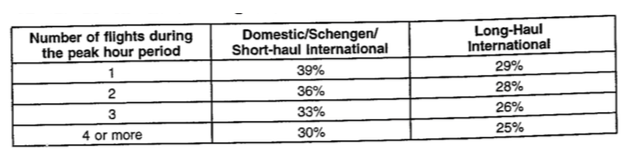
\includegraphics[width=8cm]{./images/IATA1}
\caption{F1: 30-min peak at check in as \% of PHP.}
\end{figure}

\begin{figure}[H]
	\centering
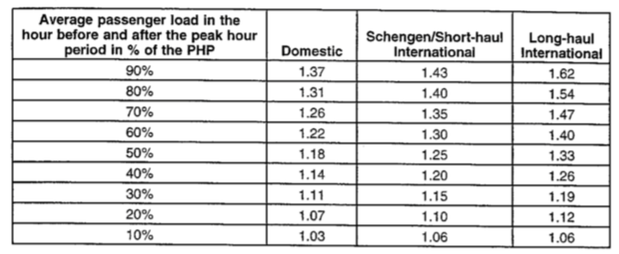
\includegraphics[width=8cm]{./images/IATA2}
\caption{F2: Additional demand based on previous and following flights to peak hour.}
\end{figure}

\begin{itemize}
\item MQT = 10 min (Maximum Queueing Time)
\item X = 810 (30-min peak at check in)
\end{itemize}

\begin{figure}[H]
	\centering
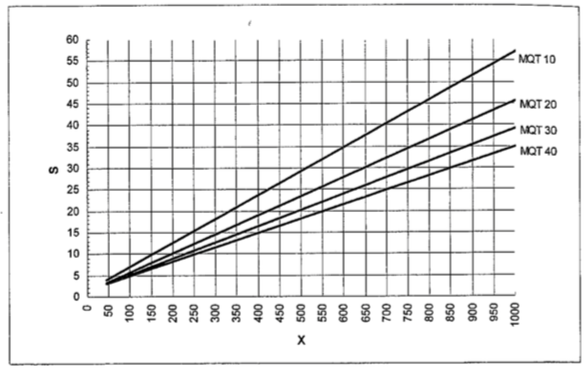
\includegraphics[width=10cm]{./images/IATA3}
\caption{Plot: S-X-MQT.}
\end{figure}

We can determine S as 49 check-in counters. Also we can add a 20\% for business class check-in counters.

\begin{align*}
\boxed{\text{\textbf{Total number of check-in counters}}= 59\text{ counters}}
\end{align*}

\item \textbf{Total passport control positions}: A multiple queue system will be used, having two accesses on each side, to reduce queues and passenger walking distances.

Considering:
\begin{itemize}
\item PHP(tot) $= 4000$ pax.
\item $b = 0 \hspace{2mm} \rightarrow$ connecting pax not processed in airside.
\item $t = 27\hspace{1mm}\mathrm{s}= 0.45\hspace{1mm}\mathrm{min} \hspace{2mm}\rightarrow$ average time per passenger in the process.
\end{itemize}

\begin{align*}
\boxed{\text{\textbf{Positions number}} = 1.1\dfrac{PHP+b}{60}\Delta t = 30}
\end{align*}

The total number of passport control positions will be 18. Since the ratio arrivals-departures is equal, the 50\% will be assigned to departures and 50\% to arrivals.


\item \textbf{Security controls:} To determine the number of x-ray machines needed, it is considered:
\begin{itemize}
\item PHP(dep) $= 2000$ pax.
\item $b = 0 \hspace{2mm} \rightarrow$ connecting pax not processed in airside.
\item $y = 600\hspace{1mm} \text{u/h} \hspace{2mm} \rightarrow$ number of units that the machine is able to process in one hour.
\item $y = 2\hspace{1mm} \text{units} \hspace{2mm} \rightarrow$ baggage items carried by passenger.
\end{itemize}

\begin{align*}
\boxed{\text{\textbf{X-ray machine number}}= \dfrac{PHP+b}{y}w = 6.666 \approx 7}
\end{align*}

A number of 7 x-ray machines are needed to give service to the airport.

\item \textbf{Health controls:} In the arrivals area, a health control is placed randomly for the passengers arriving from international flights. Considering:
\begin{itemize}
\item $t = 0.17\text{ min} \hspace{2mm} \rightarrow $ Average selecting process time.
\item $p = 400$ PAX $\rightarrow$ Number of PAX in the international critical aircraft (B777-300ER)
\item $m = 30$ min $\rightarrow$ required time to complete the control.
\end{itemize}

\begin{align*}
\boxed{\text{\textbf{Number of positions}} = \dfrac{p}{m}\Delta t \approx 3   }
\end{align*}


\item \textbf{Baggage claim area:} The dimensions of the baggage claim area, are compute according the following parameters.
\begin{itemize}
\item PHP(arr) = 2000 $\rightarrow$ arriving passengers per hour.
\item $w = 30$ min $\rightarrow$ average time per passenger.
\item $s = 1.8\hspace{1mm} \mathrm{m^2}$ $\rightarrow$ recommended area per passenger.
\begin{align*}
\boxed{\text{\textbf{Baggage claim area}} = 1.1\dfrac{aws}{60} \approx 1000 \hspace{1mm}\mathrm{m^2} }
\end{align*}
\end{itemize}

To compute the number of baggage claim belts, it is considered:
\begin{itemize}
\item $PHP$ = 1000 $\rightarrow$ arriving passengers per hour.
\item $q=0.7$ $\rightarrow$ proportion passengers in wide-body aircraft.
\item $r=0.3$ $\rightarrow$ proportion passengers in narrow-body aicraft.
\item $y=45$ min $\rightarrow$ average occupation time for wide-body aircraft.
\item $z=30$ min $\rightarrow$ average occupation time for narrow-body aircraft.
\item $n=400 \cdot 0.7$ min $\rightarrow$ number of pax in wide-body aircraft.
\item $m=200\cdot 0.3$ min $\rightarrow$ number of pax in narrow-body aircraft.
\end{itemize}

\begin{align*}
\boxed{\text{\textbf{Wide-body belts}}= \dfrac{PHP_2\cdot qy}{60n}\approx 4}
\end{align*}
\begin{align*}
\boxed{\text{\textbf{Narrow-body belts}}= \dfrac{PHP_2\cdot rz}{60m}\approx 5}
\end{align*}

The total number of baggage claim belts is 6. 

\item \textbf{Customs controls:} to determine the number of customs positions, the custom area needs to be defined.
\begin{itemize}
\item $PHP$ = 2000 $\rightarrow$ arriving passengers per hour.
\item $f=0.8$ $\rightarrow$  proportion of inspected passengers.
\item $s=1.5\hspace{1mm} \mathrm{m^2}$ $\rightarrow$ area recommended per passenger.
\item $t=2$ min $\rightarrow$ average passenger time.
\end{itemize}

\begin{align*}
\boxed{\text{\textbf{Number of customs positions}} = \dfrac{PHP\Delta f}{60}1.1\Delta t \approx 59}
\end{align*}





\end{enumerate}